\documentclass[11pt, oneside]{article} 
\usepackage{geometry}
\geometry{letterpaper} 
\usepackage{graphicx}
	
\usepackage{amssymb}
\usepackage{amsmath}
\usepackage{parskip}
\usepackage{color}
\usepackage{hyperref}

\graphicspath{{/Users/telliott_admin/Tex/png/}}
% \begin{center} 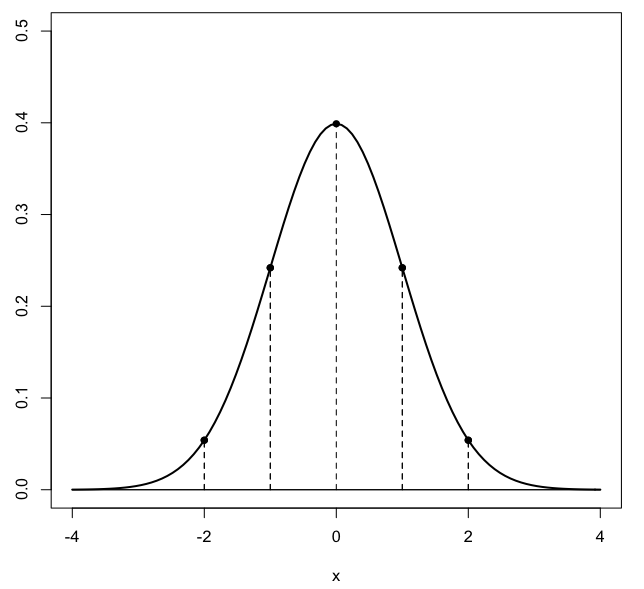
\includegraphics [scale=0.4] {gauss3.png} \end{center}

\title{Partial derivatives}
\date{}

\begin{document}
\maketitle
\Large
In calculus we start with a single variable $y = f(x)$, but the world is often more complicated than that.  For example, the Ideal Gas Law is
\[ PV = nRT \]
Considering the number of moles of gas as fixed, there are still three variables.  Pressure is a function of temperature and volume.
\[ P = \frac{1}{V} nRT \]

Or consider:
\[ f(x,y) = a^2 - x^2 - y^2 \]
where $x$ and $y$ are variables and $a$ is a constant.

We ask "how does $f$ change when $x$ and $y$ change"?  We ask the question about one variable at a time, for example about $x$ while holding $y$ constant, and write
\[ \frac{\partial f}{\partial x} = -2x \]
Since the $y^2$ term is taken to be constant when evaluating, its derivative $\partial/\partial x$ is zero.

On the other hand for
\[ f(x,y) = xy \]
\[ \frac{\partial f}{\partial x} = y \]
\[ \frac{\partial f}{\partial y} = x \]

The official definitions use the difference quotient
\[ \frac{\partial f}{\partial x} = \lim_{\Delta x \rightarrow 0} \ \frac{f(x + \Delta x, y) - f(x,y)}{\Delta x} \]
\[ \frac{\partial f}{\partial y} = \lim_{\Delta y \rightarrow 0} \ \frac{f(x,  + \Delta y) - f(x,y)}{\Delta y} \]

There is another notation for partial derivatives which I find very useful (Schey, who wrote a wonderful book on multivariable calculus, doesn't like it):
\[ f_x = \frac{\partial f}{\partial x}  \]
so
\[ \nabla f = \ \langle f_x, f_y \rangle \]
\begin{center} 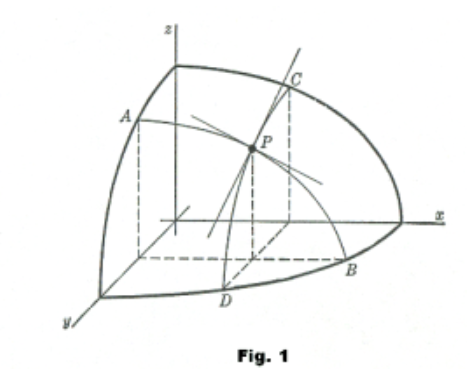
\includegraphics [scale=0.4] {gradient1.png} \end{center}
In the figure, $f_x$ is the slope of the tangent line parallel to the $x$-axis, and $f_y$ the slope parallel to the $y$-axis.
\subsection*{gradient}

It turns out that the direction in which the slope \emph{increases the fastest} is 
\[ \ \langle f_x, f_y \rangle \]
we call this the gradient of $f$ or $\nabla f$.
\[ \nabla f = \ \langle f_x, f_y \rangle \]
For example, suppose
\[ f(x,y) = xy^2 + y \]
then
\[ \nabla f = \ \langle y^2, 2xy + 1 \rangle \]
A widely used "abuse of notation" is to consider $\nabla$ as an operator with this definition in three dimensions:
\[ \nabla = \ [  \frac{\partial }{\partial x}  ] \ \mathbf{\hat{i}} +  \ [ \frac{\partial }{\partial y} ] \ \mathbf{\hat{j}} + \ [ \frac{\partial }{\partial z} ] \ \mathbf{\hat{k}} \]

\subsection*{tangent plane}
We can use the partial derivatives to get an equation for the tangent plane to the surface at a point.
\begin{center} 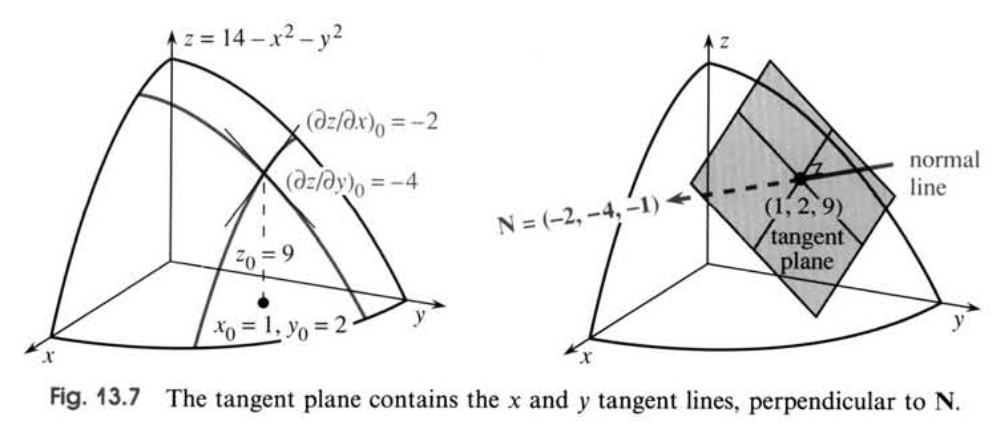
\includegraphics [scale=0.35] {tangent_plane.png} \end{center}
If we know a point $(x_0,y_0,z_0)$ where the derivatives are $f_x$ and $f_y$, then the equation of the plane tangent to the surface at that point is
\[ z - z_0 = f_x (x - x_0) + f_y (y - y_0) \]
\[ \Delta z = f_x \Delta x + f_y \Delta y \]
a rearrangement
\[ z = z_0 + f_x (x - x_0) + f_y (y - y_0) \]
is called the tangent approximation.

\subsection*{normal vector}
Consider this vector which lies in the tangent plane and has constant $y$:
\[ \mathbf{u} = \langle 1,0,f_x \rangle \]

That is the very definition of slope.  We move $1$ unit in the $x$ direction and not at all in the $y$ direction and the change in the $z$ direction is $f_x$.  The same for the orthogonal vector
\[ \mathbf{v} = \langle 0,1,f_y \rangle \]

Starting with two vectors in the plane, their cross-product is orthogonal to both, and thus is a normal vector for the plane.
\[ \mathbf{u}  \times \mathbf{v}  = \mathbf{N} = \ \langle -f_x, - f_y, 1 \rangle \]
To get the unit normal, divide by the length
\[ \mathbf{\hat{n}} = \frac{\langle -f_x, - f_y, 1 \rangle}{\sqrt{1 + {f_x}^2 + {f_y}^2}} \]

\subsection*{chain rule}
Suppose that $x$, $y$ and $z$ are all functions of some other variable, a parameter $t$.  Then the chain rule says that
\[ \frac{df}{dt} = \frac{\partial f}{\partial x} \ \frac{dx}{dt} + \frac{\partial f}{\partial y} \ \frac{dy}{dt} + \frac{\partial f}{\partial z} \ \frac{dz}{dt} \]

We might write the differential
\[ df = \frac{\partial f}{\partial x} \ dx + \frac{\partial f}{\partial y} \ dy + \frac{\partial f}{\partial z} \ dz \]
or even
\[ df = f_x \ dx + f_y \ dy + f_z \ dz \]

However, $\partial x$ by itself doesn't mean anything.

Here is an example from Strang:  suppose we have a triangle where two of the sides are $a$ and $b$ and the angle between them is $\theta$.  Then the area is
\[ A = f(a,b,\theta) = \frac{1}{2} ab \cos \theta \]
and 
\[ f_a = \frac{1}{2} b \sin \theta \]
\[ f_b = \frac{1}{2} a \sin \theta \]
\[ f_{\theta} = -\frac{1}{2} ab \cos \theta \]
then
\[ df = \frac{1}{2} b \sin \theta  \ da + \frac{1}{2} a \sin \theta  \ db + \frac{1}{2} ab \cos \theta \]

\subsection*{mixed partial derivatives}
In one dimension we get a single second derivative, but with multiple variables there are more derivatives.  Here's an example:
\[ f(x,y) = xy^2 + e^x + ye^y \]
The first derivatives are
\[ f_x = y^2 + e^x \]
\[ f_y = 2xy + e^y + ye^y \]
There are four different second derivatives:
\[ f_{xx} = e^x \]
\[ f_{yy} = 2x + 2e^y + y e^y \]
\[ f_{xy} = 2y \]
\[ f_{yx} = 2y \]

The mixed partials are equal.  It turns out that always happens.  In fact it is a tremendous help in thinking about vector fields as we'll see later.

Shankar has a great explanation of why this is true.  If we are making a small change in $x$ and a small change in $y$, we can imagine doing it by two different tiny paths:
\begin{center} 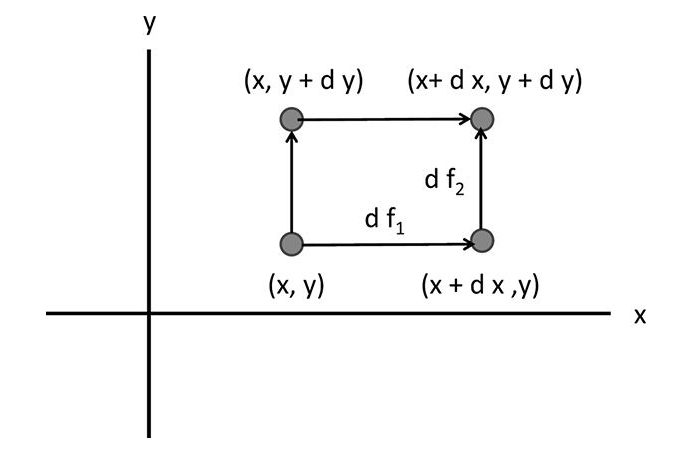
\includegraphics [scale=0.3] {mixed_partials.png} \end{center}
Here we have a view of the plane, but keep in mind the value $f(x,y)$ forms a surface above the plane in $\mathbb{R}^3$.

We can either change $x$ first and then $y$ or first $y$ and then $x$.  We need to get to the same height $z = f(x,y)$ for either path.

Write the differential for the first step from $(x,y)$ to $(x + dx, y)$ as
\[ df_1 =  f_x \ \bigg |_{(x, y)} \ dx \]
We take $f_x$ evaluated at $(x,y)$ and multiply by the change $dx$

But now the value of the function has become $f + df_1$.  It is this value which we plug into the formula to calculate the new $df_2$
\[ df_2 =  f_y \ \bigg |_{(x + dx, y)} \ dy \]
We evaluate the derivative with respect to $y$ at the new point $(x + dx, y)$ and that is what we use to multiply by the change $dy$.

As Shankar says:  "because the partial derivative is itself just another function of x and y, we may write to leading order in dx."
\[ f_y \ \bigg |_{(x + dx, y)}  = \frac{\partial}{\partial y} \ [ \ f(x, y) \ ] \ + \frac{\partial}{\partial y} \ [ \ f_x \ dx ]  \]
\[ = f_y \ \bigg |_{(x, y)} + f_{xy} \ \bigg |_{(x, y)} \ dx \]
By $f_{xy}$ we understand that the derivative with respect to $y$ is taken second.

So now when we take the step up, from the \emph{new} point we make the change in $z$ as
\[ df_2 =  f_y \ \bigg |_{(x + dx, y)} \ dy \]
\[ = f_y \ \bigg |_{(x, y)} \ dy + f_x f_y \  \ \bigg |_{(x, y)} \ dx \ dy \]
and combining the two terms
\[ df = df_1 + df_2 \]
\[ =   f_x \ \bigg |_{(x, y)} \ dx + f_y \ \bigg |_{(x, y)} \ dy + f_{xy} \ \bigg |_{(x, y)}  \ dx \ dy \]

The insight is that if we had gone by the other path we would have the same thing (with the first two terms switched) except the last term would be
\[  f_{yx} \ dy \ dx \]
But these must be equal:
\[  f_{xy}\ dx \ dy = df = f_{yx} \ dy \ dx \]
Hence
\[  f_{xy} = f_{yx} \]
And that's worth remembering.

\end{document}